\chapter{Baseline setup}

\section{Overview}

\begin{figure}[h]
	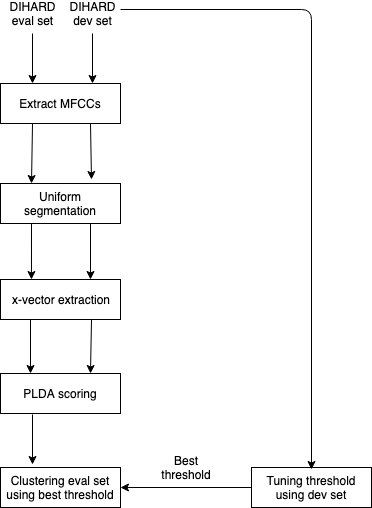
\includegraphics[width=9cm]{figures/baseline.png}
	\centering
	\caption{Block diagram of DIHARD diarization baseline.}
	\label{fig:fig-baseline}
\end{figure}

There are three software baselines provided by the DIHARD II organizers, each for the parts of speech enhancement, speech activity detection and diarization. The speech enhancement baseline and the speech activity detection are meant to be used together in the case of system-generated SAD (tracks 2 and 4), but since we only work with reference SAD, we do not need them. Thus we will only describe the diarization baseline in the following sections.

The diarization baseline is based on the best performing submission \cite{sell2018diarization} from John Hopkins University (JHU) in the previous year's DIHARD challenge (DIHARD I). There are 4 Kaldi recipes, each for an evaluation track, but we will focus only on the recipe for Track 1 since we only work with single channel audio and gold speech segmentation.

\section{Baseline directory structure}
The baseline repository is localted at \ttvar{https://github.com/iiscleap/DIHARD_2019_baseline_alltracks} and has the following directory structure. Some of the irrrelevant files have been removed.

\begin{verbatim}
DIHARD_2019_baseline_alltracks/
|-- data
|   |-- final.raw
|   |-- max_chunk_size
|   |-- min_chunk_size
|   |-- plda_track1
|   |-- plda_track2
|   |-- plda_track3
|   |-- plda_track4
|-- README.md
|-- recipes
|   |-- track1
|   |-- track2
|   |-- track2_den
|   |-- track3
|   |-- track4
|   `-- track4_den
|-- scripts
|   |-- alltracksrun.sh
|   |-- flac_to_wav.sh
|   |-- make_data_dir.py
|   |-- md_eval.pl
|   |-- prepare_feats.sh
|   |-- prep_eg_dir.sh
|   `-- split_rttm.py
`-- tools
    |-- env.sh
    |-- install_dscore.sh
    |-- install_kaldi.sh
}
\end{verbatim}

The \ttvar{data} directory has pre-trained models (in Kaldi binary format) and some configuration parameters - \ttvar{final.raw} is the neural network x-vector extractor, and the \ttvar{plda_*} files are the PLDA backends for the 4 tracks. The \ttvar{recipes} directory has the \ttvar{run.sh} files for all 4 recipes, we only care about \ttvar{track1}. The scripts directory has extra scripts that are needed on top of the \ttvar{egs/dihard_2018} Kaldi recipe - \ttvar{alltracksrun.sh} is the main diarization script, \ttvar{make_data_dir.py} makes the Kaldi data directory from the DIHARD datasets (creating files like wav.scp, segments, utt2spk etc), \ttvar{prep_eg_dir.sh} copies the extra files from this repository to the \ttvar{egs/dihard_2018} directory, \ttvar{md_eval.pl} \cite{mdeval2006} is a diarization evaluation script that was developed by NIST, and others are self-explanatory. The \ttvar{tools} directory holds scripts to install Kaldi and dscore \cite{dscore}, which are installed in the same directory.

The baseline code modifies and reuses the \ttvar{egs/dihard_2018} recipe that was checked into Kaldi by the researchers at JHU. It does this by copying over new scripts and data that is needed to the \ttvar{egs/dihard_2018} directory, \ttvar{cd}'ing to that directory and running the recipe from there.

We modify and add scripts in this repository so we can easily run experiments with different parameters. The \ttvar{run.sh} script is modified to allow easily changing parameters to run different experiments.

\section{Initial segmentation}
The initial segmentation step is done by \ttvar{make_data_dir.py}. It deals with separating speech and non-speech segments from the recording files using the reference SAD which is provided in the form of HTK label files (.lab). Each audio recording has one label file. The label file has one line for each speech segment with the format \ttvar{<start-timestamp> <end-timestamp> speech}.

\begin{verbatim}
0.000 3.513 speech
4.698 7.133 speech
7.377 12.826 speech
13.284 16.797 speech
17.312 21.201 speech
...
\end{verbatim}

This results in a bunch of segments which are known to be containing only speech. These are treated as ``utterances" in Kaldi terminology and act as keys in the \ttvar{utt2spk}, \ttvar{feats.scp} and \ttvar{segments} files. These files reside in two Kaldi ``data directories", one for each dev and eval.

\section{Features}
The baseline then extracts 30 dimensional MFCC features for each of the every 10 ms using a 25 ms window. It uses the standard \ttvar{steps/make_mfcc.sh} Kaldi script for this. The MFCC configuration used \ttvar{mfcc.conf} is given below.

\begin{verbatim}
--sample-frequency=16000
--frame-length=25 # the default is 25
--low-freq=20 # the default.
--high-freq=7600 # Nyquist (8k in this case).
--num-mel-bins=30
--num-ceps=30
--snip-edges=false
\end{verbatim}

Later, cepstral mean and variance normalization (CMVN) with a 3 second sliding window is applied using the \ttvar{apply-cmvn-sliding} Kaldi tool.

\section{Subsegmentation}
After MFCC features are ready, the utterances are uniformly divided into smaller 1.5 second subsegments with a 0.75 second overlap. This creates new Kaldi data directories (one each for dev and eval sets) with newer keys corresponding to each subsegment. An x-vector is extracted from each of these subsegments in the next step using the Kaldi binary \ttvar{nnet3-xvector-compute}.

\section{Speaker representation}
The baseline extracts an 512-dimensional x-vector from each subsegment using a neural network x-vector extractor. The extractor is trained on the datasets VoxCeleb I and II, along with added augmentation. Utterances smaller than 400 frames and speakers less than 8 utterances are discarded. Since the VoxCeleb dataset does not come with gold speech segmentation, the program \ttvar{compute-vad} is used with the following configuration to classify each frame into speech or non-speech.

\begin{verbatim}
--vad-energy-threshold=5.5
--vad-energy-mean-scale=0.5
--vad-proportion-threshold=0.12
--vad-frames-context=2
\end{verbatim}

It uses simple energy-based thresholding to generate a speech segmentation. Finally there are 1,277,503 utterances spoken by 7,351 speakers that can be used for training. Although the actual number is much more because of augmentation.

The augmentation is done by additive noise (noise, music, babble) using the MUSAN dataset and reverberation using the RIR dataset. The augmentation is done because it was determined in \cite{snyder2018x} that x-vectors exploit large quantities of training data much better than i-vectors, and show a significant increase in performance.

\section{Scoring}
For scoring two x-vectors, a PLDA backend is used as a distance metric. To train the PLDA backend, x-vectors are extracted from a random subset (size 128k) of the VoxCeleb dataset. To adapt the extracted x-vectors to the DIHARD domain, they are whitened with a whitening transform learned from the DIHARD development set. The PLDA model is trained using the x-vectors and the \ttvar{ivector-compute-plda} Kaldi binary.

Each pair of x-vectors within a recording is then scored using the PLDA backend by reusing \ttvar{score_plda.sh} from \ttvar{egs/callhome_diarization}. These scores are stored as an affinity matrix for each recording.

\section{Clustering}
The x-vectors are then clustered using agglomerative hierarchical clustering (AHC) and a parameter sweep is done on the dev set to find the threshold that maximises the DER on the dev set. This threshold is then used for clustering the x-vectors of the eval set. The \ttvar{agglomerative-cluster} Kaldi binary is used for clustering.

\section{Diarization output}
The clustering output is used to generate RTTMs using the script \ttvar{make_rttm.py} from \ttvar{egs/callhome_diarization}. The RTTMs give a flat segmentation of the recordings with no overlap. Since the x-vectors were extracted from segments that were overlapping, care needs to be taken when two adjacent segments are assigned to a different speaker. The script places the speaker boundary midway between the end of the first segment and the start of the second segment.

